\section{Installation Coordination and Support}
\label{sec:fdsp-coord-install}
%						15 pages

%%%%%%%%%%%%%%%%%%%%%%%%%%%%%%%%
%\subsection{Organization}
%\label{sec:fdsp-coord-org}

Installation Coordination and Support %or 
(also called simply \textit{Installation}) is
responsible for coordinating the detector installations, providing
detector installation support and providing installation-related
infrastructure. The installation group management responsibility is
shared by a scientific lead and a technical lead that report to the
Technical Coordinator. The %underground 
group responsible for activities in the underground areas is referred to as
the \dword{uit}. The \dword{itf} group, which delivers equipment to the
Ross Shaft, and the \dword{uit}, which receives the equipment
underground, need to be in close communication and work closely
together.

Underground installation is in general responsible for coordinating
and supporting the installation of the \dwords{detmodule} and providing
necessary infrastructure for installation of the experiment. While the
individual consortia are responsible for the installation of their own
detector equipment, it is essential that the detector installation be
planned as a whole and that a single group coordinates the
installation and adapts the plans throughout the installation
process. The \dword{uit} has responsibility for overall coordination
of the installations. In conjunction with each consortium the
\dword{uit} makes the installation plan that describes how the
\dwords{detmodule} are to be installed. The installation plan is used to define
the spaces and infrastructure that will be needed to install them.
%detectors. 
The installation plan will also be used to define the
interfaces between the Installation group and the consortium
deliverables.

\subsection{UIT Infrastructure}

The installation scope includes the infrastructure needed to install
the \dword{fd} such as the cleanroom, a small machine shop, special
cranes, scissor lifts, and access equipment.  Additional equipment
required for installation includes: rigging equipment, hand tools,
diagnostic equipment (including oscilloscopes, network analyzers, and
leak detectors), local storage with some critical supplies and some
personal protective equipment (PPE). The \dword{uit} will also provide
trained personnel to operate the installation infrastructure. The
consortia will provide the detector elements and custom tooling and
fixtures as required to install their detector components.




%%%%%%%%%%%%%%%%%%%%%%%%%%%%%%%%
\subsection{Underground Detector Installation}
\label{sec:fdsp-coord-undergd}

For the \dwords{detmodule} to be installed in safe and efficient
manner, the efforts of the individual consortia must be coordinated
such that the installation is planned as a coherent process. The
interfaces between the individual components must be understood
and the spaces required for the installation process planned and
documented. The installation planning must take into account the
plans and scope of the \dword{lbnf} effort and the individual plans of
the nine consortia. By working with the \dword{lbnf} team and the
members of the consortia responsible for building and installing their
components, a joint installation plan and schedule, taking into account
all activities and needs of all stakeholders, can be developed. Although
the organization of the installation effort is still evolving, 
an installation coordinator will be the equivalent of a scientific lead for this effort.

One of the primary early responsibilities of the \dword{uit} is to
develop and maintain the \dword{dune} installation plan and the
installation schedule. This installation plan 
describes the installation process in sufficient detail to demonstrate
how all the individual consortium installation plans mesh and it 
gives an overview of the installation process. The installation plan
is used by the \dword{uit} to define the underground infrastructure
needed for detector installation and the interfaces it has with respect  to 
the consortia. The \dword{uit} is responsible for reviewing and
approving the consortium installation plans. Approved installation
plans, engineering design notes, signed final drawings, and safety
documentation and procedures are all prerequisites for the \dword{prr}. 
Approved procedures, safety approval, and
proper training are all required before the \dword{uit} performs
work. During the installation phase the installation leadership 
coordinates the \dword{dune} installation effort and adapts the schedule
as needed. The installation coordinator, together with management, will also
resolve issues when problems occur.

The installation infrastructure to be provided by the \dword{uit}
includes: the underground ISO 8 (or class \num{100000}) clean room
used for the installation; cranes and hoists (if they are not
delivered by \dword{lbnf}); and scissor lifts, aerial lifts, and the common
work platforms outside the cryostat. The \dword{uit} will have
responsibility for operating this equipment and assisting the
consortia with activities related to rigging, material transport, and
logistics. Each consortium is responsible for the installation of
their own equipment, so the responsibility of the installation group is
limited, but the material handling scope is substantial. To support
the installation process, an installation floor manager will lead a
trained crew with the main responsibility of transporting the
equipment to the necessary location and operating the cranes, hoists,
and other common equipment needed for the installation. It is expected
that the installation crew will work with the teams from the various
consortia but will mainly act in a supporting function. The
\dword{uit} floor manager will be responsible for supervising the
\dword{uit} crew, but the ultimate responsibility for all detector
components remains with the consortia even while the underground
team is rigging or transporting these components.  This will be
critical in the case where any parts are damaged during transport or installation,
as the consortia need to judge the necessary actions. 
\fixme{judge the situation and determine the necessary actions?}
For this reason,
a representative or point of contact (POC) from the consortia must be
present when any work is performed on their equipment. The consortium
is responsible for certifying that each installation step is properly
performed.

The \dword{uit} acts as the primary point of contact with
\dword{lbnf} and \surf from the time the components reach the Ross
headframe until the equipment reaches the experimental cavern. If
something goes wrong, \surf calls the \dword{uit} leader who then
contacts the responsible party. The consortia are responsible for
delivering to the \dword{uit} all approved procedures and specialized
tooling required for transport. The \dword{uit} leader acts as a point
of contact if the \dword{lbnf} or \surf team has questions or difficulties
with the underground transport.  The \dword{uit} receives the
materials from \dword{lbnf} and \surf at the entrance to the \dword{dune}
excavations. The \dword{uit} then delivers the equipment to the
required underground location.

In an effort to get an early estimate of the equipment required to
install the detectors the \dword{uit} has developed a preliminary
installation plan that outlines the installation process. At present
the installation plan consists of a \threed model of the cryostat in the
excavations. The \dword{spmod} elements are inserted in the
model and a proposal for how they are transported, assembled, and
inserted into the cryostat has been conceptually developed and expressed in a series of images
some of which are shown in Figures~\ref{fig:Install-seq} and~\ref{fig:cpa-fc-unpack-assy}. 
%
Conceptual designs of the infrastructure needed to support
the transport and assembly are also included in the model. See Figures~\ref{fig:Install-ISO-Top} and~\ref{fig:Install-TopView}. With this
as a tool, the proposed installation sequence can be iterated with the
consortia to converge on a baseline installation plan. A similar
process will be followed for the \dword{dpmod} once the base
configuration for the \dword{sp} installation is agreed upon. The
\dword{uit} has focused initially on the \dword{spmod} as the
\dword{sp} components are larger and the installation process more
complex. 

\begin{dunefigure}[APA and CPA installation steps]{fig:Install-seq}
  {Top row from left:  crated \dword{apa} rotating to vertical position;  crated vertical \dword{apa} placed in cart; \dword{apa} panels moved to fixture using the under-bridge crane. Bottom row: series showing \dword{cpa} panels uncrated and moved to fixture. }
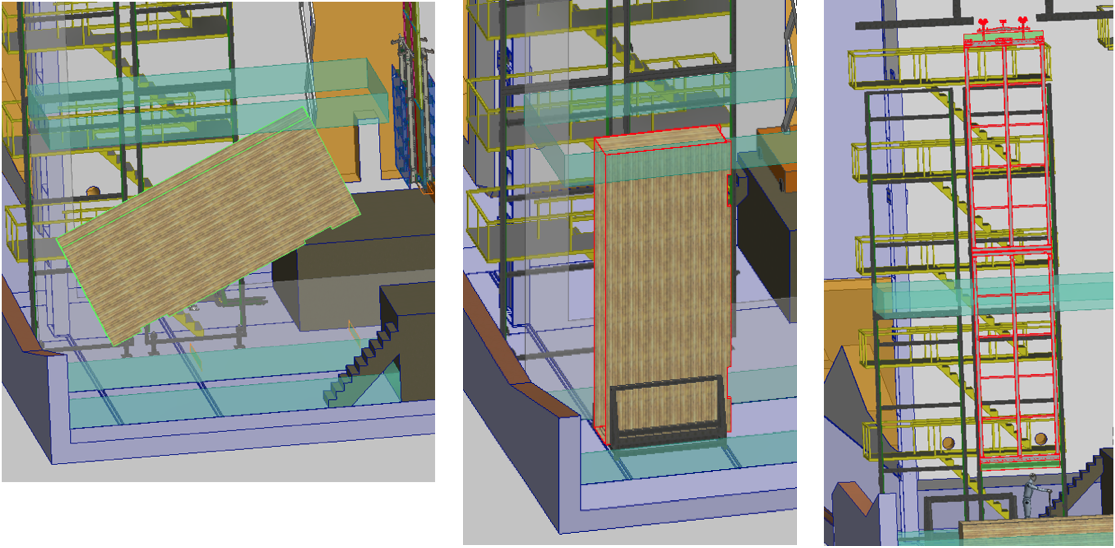
\includegraphics[width=.9\textwidth]{apa-install-seq-top}
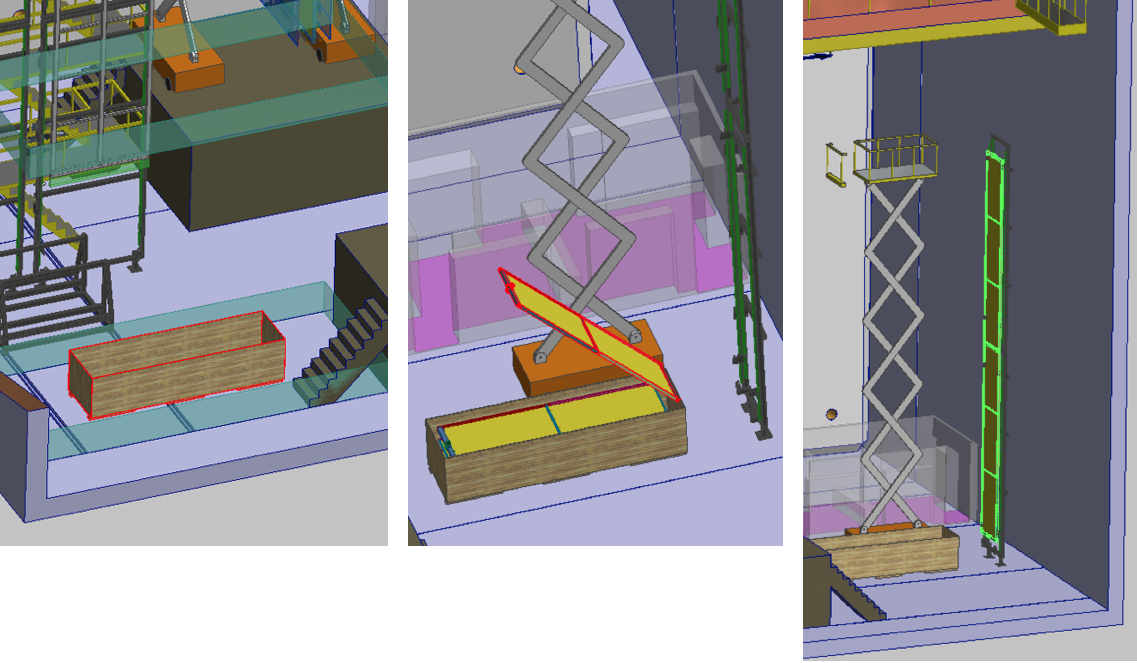
\includegraphics[width=.9\textwidth]{cpa-install-seq-bot}
\end{dunefigure}

\begin{dunefigure}[\dword{cpa} and \dword{fc} unpacking and assembly]{fig:cpa-fc-unpack-assy}
  {On the left, the assembled \dword{cpa} panel is placed onto the north \dword{tco} beam. On the right, the (green) \dword{fc} panels (already lowered into \dword{sas} and moved into the clean room) are installed as the \dword{cpa} array hangs under the \dword{tco} beam. }
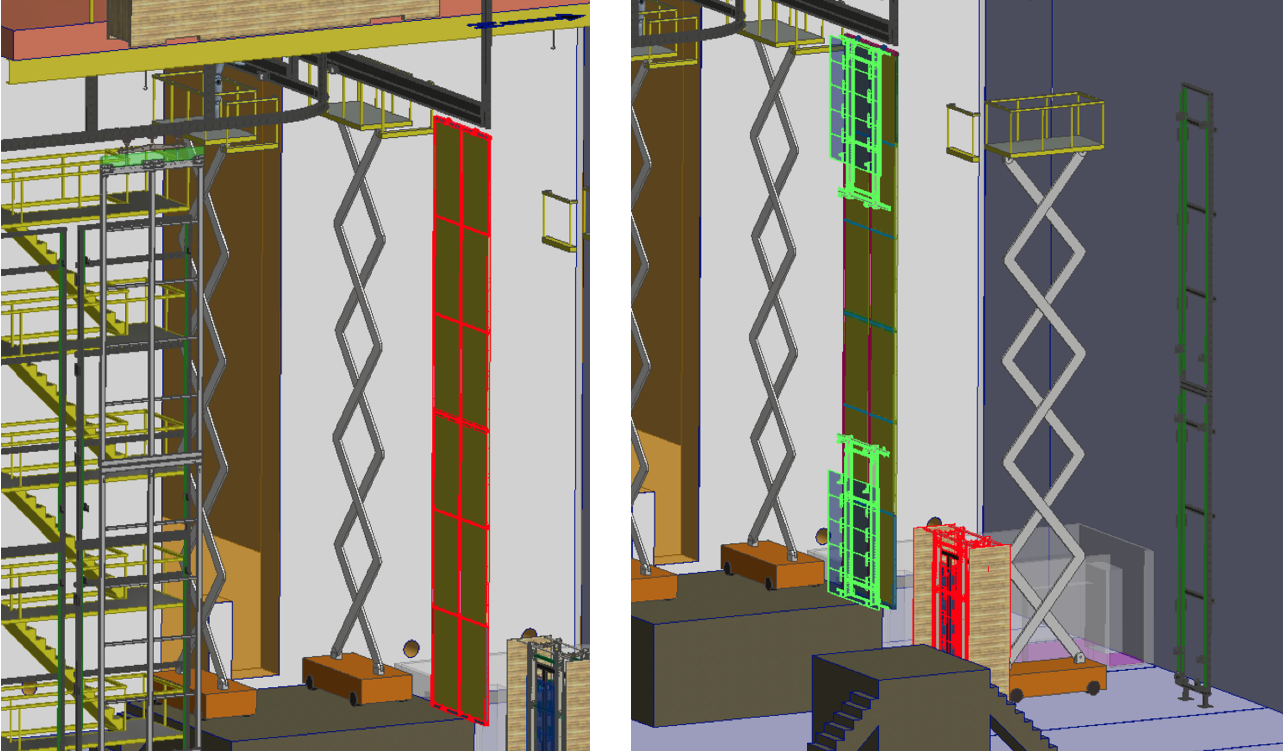
\includegraphics[width=.9\textwidth]{cpa-fc-unpack-assy}
\end{dunefigure}

\begin{dunefigure}[\threed model of underground area showing installation infrastructure]{fig:Install-ISO-Top}
  {\threed model of the underground area showing the infrastructure to install the \dword{spmod} in cryostat~1. The most significant features are presented including the \dword{apa} and \dword{cpa} assembly areas, the region around the \dword{tco} for materials entering the cryostat,  the changing room, the region for the materials air lock, (\dword{sas}), 
  and the means of egress.}
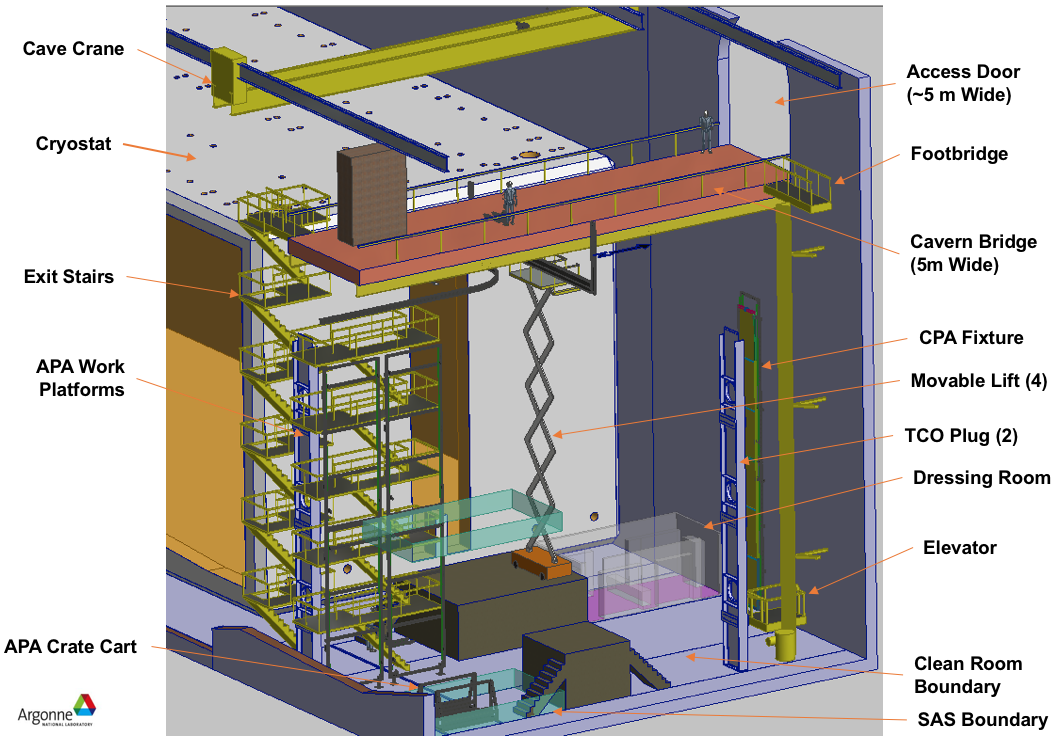
\includegraphics[width=.9\textwidth]{Install-ISO-Top}
\end{dunefigure}

\begin{dunefigure}[Section view of the \threed model showing layout]{fig:Install-TopView}
  {Section view of the \threed model showing layout, looking down on the installation area from below the bridge. Areas shown, left to right,  are the cryostat and \dword{tco}, the platform in front of the \dword{tco}, the dressing area, the \dword{apa} and \dword{cpa} assembly area (directly under the bridge), and the stairs and elevator. The lower right corner of the region is used as the materials air lock.}
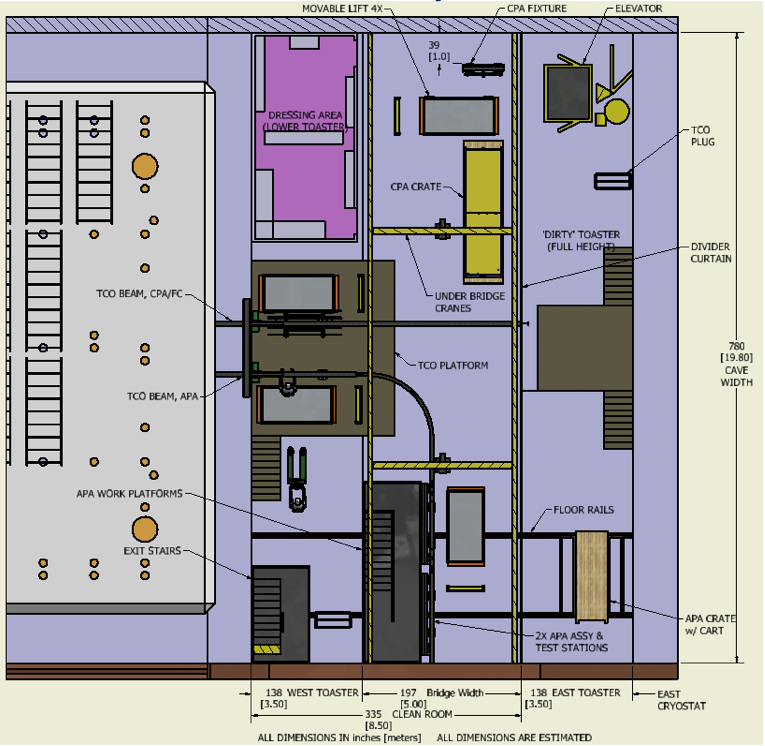
\includegraphics[width=.9\textwidth]{Install-TopView}
\end{dunefigure}





%The current installation plan is described. 
In the current installation plan, \dword{dune} will take
ownership of the different underground areas at different times. The
surface data room and the underground room in the \dword{cuc} are available
significantly before the collaboration has access to the cryostats; 
the optical fibers between the surface and underground will be in
place even earlier. This will allow a \dword{daq} prototype to be developed
and tested early. The installation of the \dword{daq} hardware can also be
finished before the start of detector installation if desired, so the
\dword{daq} will not be on the critical path.  When the collaboration receives
access to Cryostat~1 the steel work for Cryostat~2 will be
finished and the work on installing the membrane will have
started. Excavation will be complete.  For planning purposes it is
assumed that the first \dword{detmodule} will be \dword{sp} and the second
\dword{dp}. The first step in the \dword{sp} installation is to
install the cryogenics piping and the \dword{dss}. As this piping will
require welding and grinding, it is a dirty process and must be
complete before the area can be used as a clean room. When this is
complete the cryostat can be cleaned and the false floor
re-installed. The clean infrastructure for installing the \dword{detmodule},
including the clean room, work platforms, scaffolding, the
fixturing to hold the detector elements during assembly, and all the
lifts need to be set up. Once the infrastructure is in place and the
area is clean, the installation of the main elements can start. The
general layout of the installation area showing the necessary space
and equipment is shown in Figure~\ref{fig:Install-seq}. 

The \dword{spmod}  is installed by first installing the west endwall or
endwall~1 (see Figure~\ref{fig:endwall}).

\begin{dunefigure}[End view of \dword{spmod} with \dword{ewfc} in
  place]{fig:endwall}
  {End view of \dword{spmod} with \dword{ewfc} in
  place, with one row of \dwords{apa} and \dwords{cpa}.}
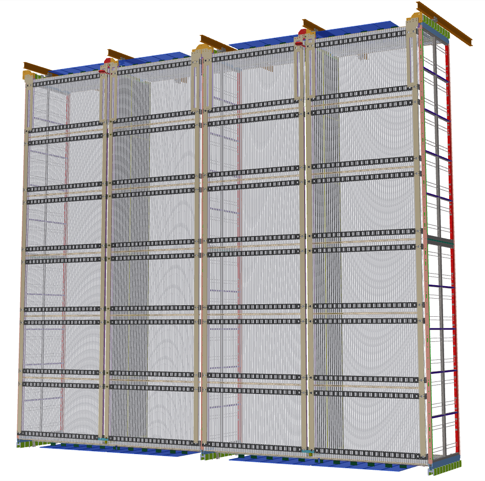
\includegraphics[width=0.6\textwidth]{endwall.png}
\end{dunefigure}

The \dwords{apa} and \dwords{cpa} with top and bottom \dword{fc} panels are
installed next. The plan is to install six \dwords{apa} and four
\dwords{cpa} per week, which is enough to complete one of the \num{25}
rows every week. Additional time is built into the schedule to take
into account that the installation will be slower at the beginning and
some re-work may be needed. By building west-to-east, complete rows can
be finished and tested before moving to the next row. This reduces the
risk of finding a fault after final \dword{fc} deployment and cabling,
which would require dismantling part of the \dword{detmodule}. Some of the steps
needed to install the \dword{apa} and \dword{cpa} modules outside the
cryostat are also shown in Figure~\ref{fig:Install-seq}.  The middle three
panels show how the \dword{apa} needs to be handled in order to rotate
it and mount it to the assembly frame. After two \dwords{apa} are
mounted on top of each other, the cabling for the lower \dwords{apa}, and the
\dword{ce} and \dword{pd} cables can be installed. The
lower three panels show how the \SI{2}{m} \dword{cpa} sub-panels are
removed form the transport crates and assembled on a holding frame. Once
the \dword{cpa} module is assembled the \dword{fc} units can be
mounted. Finally, once the \dwords{apa} and \dwords{cpa} are installed,
the endwall~2 can be installed. A high-level summary of the schedule
is shown in Figure~\ref{fig:Install-Schedule}.

\begin{dunefigure}[High-level installation schedule]{fig:Install-Schedule}
  {High-level installation schedule.}
 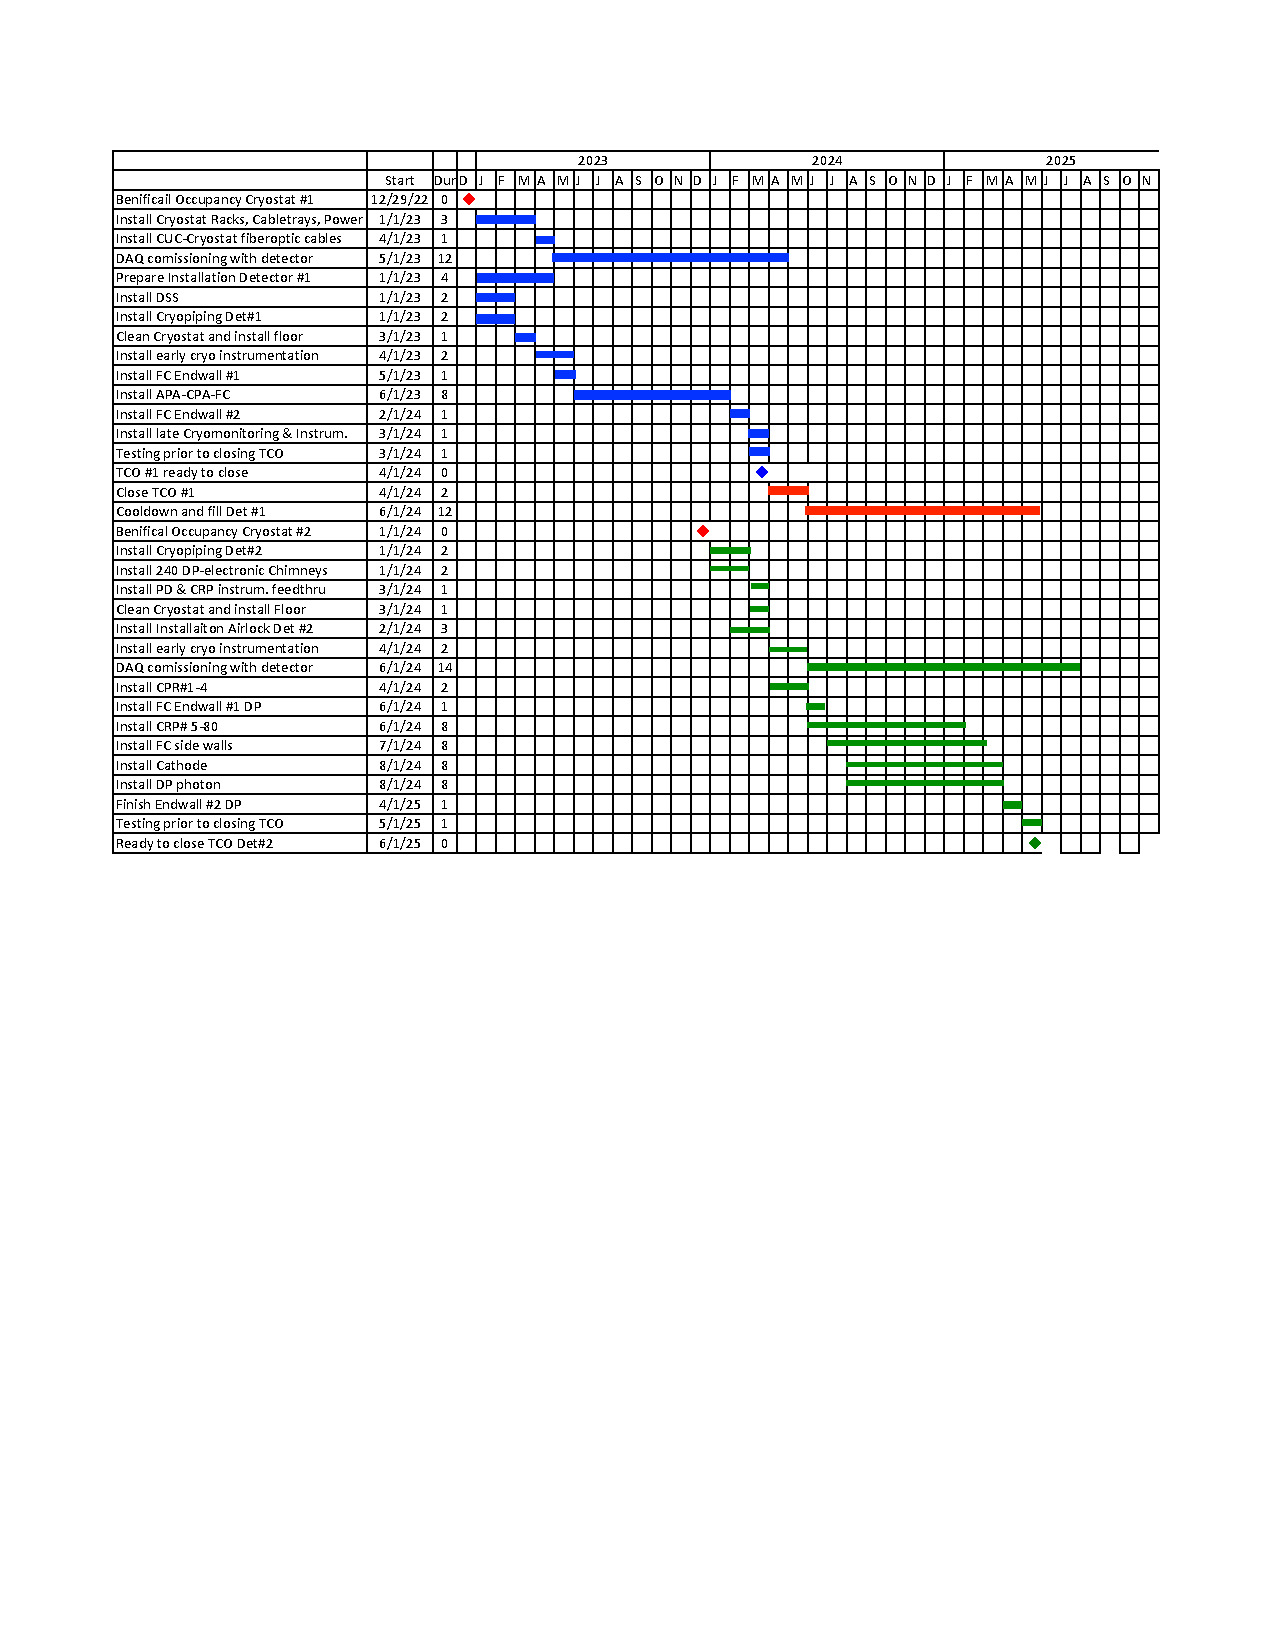
\includegraphics[width=\textwidth]{TP-Schedule-Feb2018.pdf}
\end{dunefigure}


As is seen in the installation schedule the second cryostat becomes
available four months before the first \dword{detmodule} installation is
complete. In this period, installation work for both \dwords{detmodule} 
proceeds in parallel. Like the \dword{spmod}, the first step is
the installation of the cryogenics piping, followed by a thorough cleaning
and installation of the false floor. While this piping is being
installed, the \dword{dp} chimneys for the electronics along with the
\dword{pds} and \dword{crp} instrumentation \fdth{}s can also be installed. Since the
chimneys are installed into the roof of the cryostat,  this work is
performed well away from the final installation work on the first
\dword{detmodule} so there should be no conflicts. Once the first \dword{detmodule} is
installed work on setting up the second \dword{detmodule}'s installation
infrastructure can begin. This work includes moving the cranes and
work platforms along with moving the walls of the clean room so that the
second cryostat is clean. The air filtration to the cryostat is also
moved to the second cryostat.  Since much of the work for the \dword{dp}
installation will be performed inside the cryostat, in principle, outside the cryostat a
clean room area smaller than that for the \dword{spmod}  would suffice. % is needed. 
However, for
planning purposes, it will not be completely clear what type of \dword{detmodule}
will be installed in the second cryostat until fairly late. Therefore the \dword{uit}
will plan to provide a sufficiently large area outside the cryostat to
accommodate either detector technology.  %The \dword{dp} detector itself
%would require 
The much smaller clean room for a \dword{dpmod} %which 
could be installed just
outside the \dword{tco}. The installation process inside the \dword{dpmod} will
proceed east-to-west. At the start of the TPC installation the first
four \dwords{crp} -- comprising the first row -- will be installed. % which comprises the first row of CRP. 
The left panel in Figure~\ref{fig:CRP-Install} shows two \dwords{crp}
being installed near the roof of the cryostat and the right panel
shows one of the \dwords{crp} in a transport box being moved into the cryostat.
Once the first \dword{crp} row is installed and tested, %then 
the first \dword{ewfc} can be installed.%In general rows of \dwords{crp} will be installed and then behind them rows of field cage modules are installed followed by the cathode installation at the bottom of the detector and the photon detector PMTs under the cathode plane. 
In general rows of \dwords{crp} will be installed, followed by rows of \dword{fc} modules, followed by the cathode installation at the bottom of the \dword{detmodule}, followed by 
\dwords{pd} under the cathode plane. 
At the end of the installation, the second \dword{ewfc} is
installed and a final testing period for the full \dword{detmodule} is
foreseen. The \dword{dpmod} installation sequence is shown in green in
Figure~\ref{Install-Schedule}.

\begin{dunefigure}[Image of the \dual CRPs being installed in
  the \dword{dpmod}]{fig:CRP-Install}
  {Left: Image of the \dword{dp} \dwords{crp} being installed in
  the \dword{dpmod}, showing the connection from the \dword{crp} to the
  electronics readout chimney. Right: Image of the \dword{crp} being
  inserted into the cryostat using a transport beam.  The \dual \dword{fc} modules will be inserted in a similar fashion.}
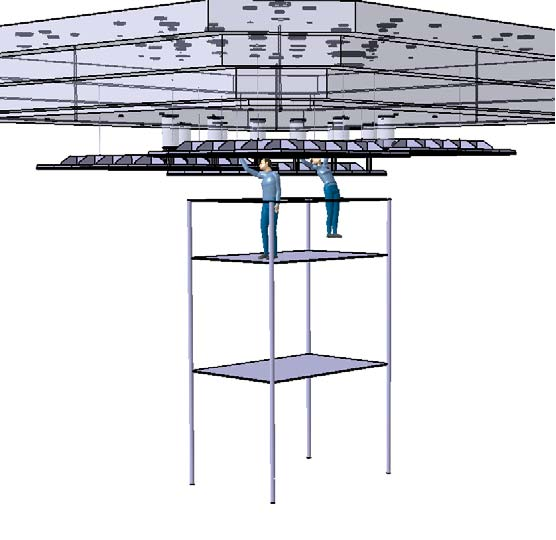
\includegraphics[width=0.45\textwidth]{CRP-install.pdf}
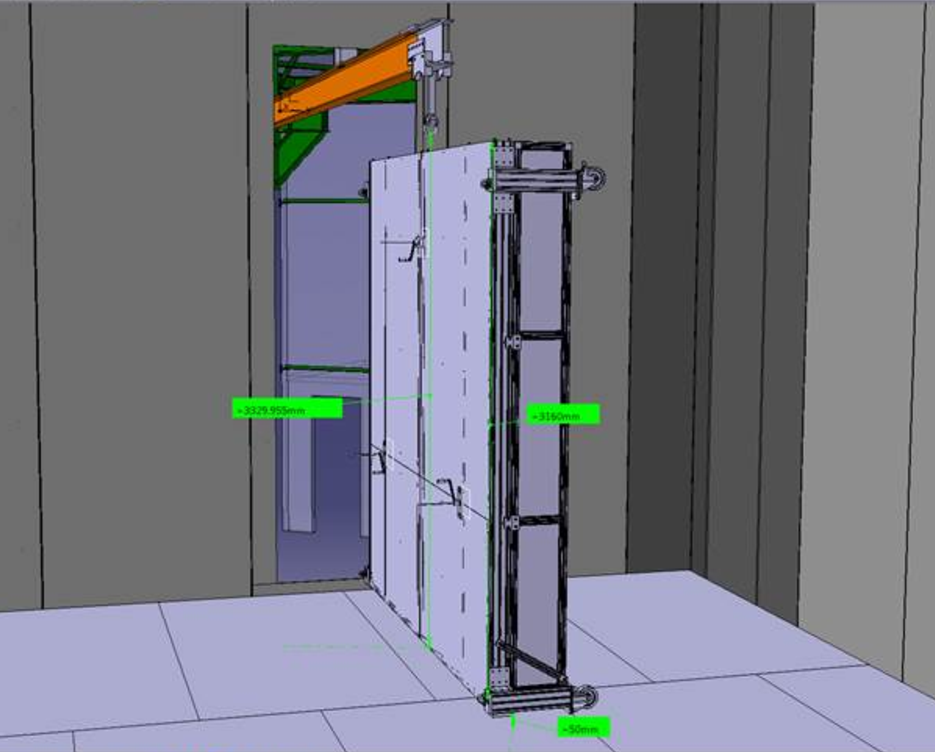
\includegraphics[width=0.45\textwidth]{CRP-into-cryostat.pdf}
\end{dunefigure}

Prior to the \dword{tdr}, mutually agreed upon installation plans must
be approved. These will set the schedule for the installation and will
determine the planning for staffing and budget. Having good estimates
for the time needed and having enough experience to ensure that the
interfaces are understood and the procedures are complete is important
for accurate planning. The experience at \dword{protodune} will be
very important as the \dword{protodune} installation establishes the
procedures for handling all the detector elements and in many cases
gives accurate estimates for the time needed. However, in the case of
the \dword{spmod}, many of these procedures need to revised or
newly developed. For example, the \dword{spmod} will be twice as high as
\dword{pdsp}, so two \dwords{apa} need to be assembled together
and a totally different cabling scheme is needed. Testing the
cabling must be done prior to the \dword{tdr} %as this is needed 
in order to
ensure the design is viable. The \dword{dp} will also need to develop
installation procedures as the \dword{dpmod} 
will have a significantly different \dword{fc} and cathode plane. 

By definition, the installation  is on the critical path, making it vital
that the work be performed efficiently and in a manner that has low
risk. In order to achieve this, a prototype of the installation
equipment for the \dword{spmod}  will be constructed at Ash
River (the \nova neutrino experiment \dword{fd} site in Ash River, Minnesota, USA), and the installation process tested with dummy detector
elements. It is expected that the setup will be available at the time
of the \dword{tdr}, but any lessons learned will need to be implemented and
tested after this. In the period just prior to the start of
installation, the Ash River setup will be used as a training ground for
the \dword{uit}.



%\subsection{Detector Support}

The Detector Support System (DSS) provides the structural support for
the single-phase detector inside the cryostat.  It also provides the
necessary infrastructure to move the detector elements into location
during assembly. As the DSS is a new design and is quite different
from the ProtoDUNE DSS it is described in some detail in this
section. The detector elements supported by the DSS include the field
cage endwalls, the \dwords{apa}, and the \dwords{cpa} with top and
bottom field cage panels.  The DSS is supported by the cryostat outer
steel structure through a series of feedthrus which cross through the
cryostat insulation and are anchored with flanges on the cryostat
roof. Inside the cryostat a series of stainless steel I-beams are
connected to the feedthrus and used to support the detector. The DSS
defines the location of the detector inside the cryostat and it also
defines how the detector elements move/contract as the detector is
brought to \dword{lar} temperature. The design of the DSS encompasses
the overall structural design of the detector as only after the
elements are mounted to the DSS and are connected together do they
make a unified mechanical structure. The requirements of the DSS are
as follows:
\begin{itemize}
 \setlength\itemsep{1mm}
\setlength{\parsep}{1mm}
\setlength{\itemsep}{-5mm}
% \small
\item Support the weight of the detector.
\item Accommodate the cryosat roof movement during cryostat filling, testing, and operation.
\item Accommodate variation in the feedthrough locations and
  variation in the flange angles due to installation tolerances and
  loading on the warm structure.
\item Accommodate shrinkage of the detector and DSS from ambient
  temperature to \dword{lar} temperature.
\item Define the position of the detector components relative to each other. 
\item The DSS is electrically connected to the cryostat ground and electrically isolated from the detector.
\item The DSS support penetrations must be purged with GAr to prevent contaminants from diffusing back into the liquid
\item The instrumentation cabling must not interfere with the DSS.
\item The DSS components must be able to be installed through the TCO
\item The DSS is to designed to meet AISC-360 and appropriate codes required by SURF
\item The DSS will be designed to meet seismic requirements 1 mile underground at SURF
\item All materials must be compatible for operation in ultrapure \dword{lar}
\item The DSS beams will be completely submerged in \dword{lar}
\item The DSS will ensure that detector components shall not be less than \SI{400}{mm} from the membrane flat surface
\item The DSS supports shall not interfere with the cryostat I-beam structures
\item The DSS shall be designed such that it supports the detector so that the lower ground plane is above the cryogenic piping and the top of the DSS beams are submerged in \dword{lar} while leaving a 4\% ullage at the top of the cryostat.
\item The DSS shall have infrastructure necessary to move the \dword{apa} and \dword{cpa}-FC assemblies from outside the cryostat through the TCO and to the correct position.
\end{itemize}

Figure~\ref{DSS} (left) shows the DSS structure; there are five rows
of supports for the alternating rows
of \dword{apa}-\dword{cpa}-\dword{apa}-\dword{cpa}-\dword{apa}.  The
DSS is connected to the warm structure at a flange that is mounted on
the outside of the cryostat.  Figure~\ref{DSS} (right) shows the
layout of these structural feedthroughs.  The DSS consists of pairs of
feedthroughs that support \SI{6.4}{m}-long S8x18.4 stainless steel I-beam
sections. The proposed design of the DSS has \num{10} I-beam segments per
row for a total of \num{50} I-beam segments. Each I-beam is suspended on
both ends by rods from feedthroughs that penetrate the roof.  In the
cold condition each beam will shrink which will cause gaps to form
between \dwords{apa} that are adjacent but supported on separate
beams.  \dwords{apa} that are supported on the same beam will not have
gaps develop because both the beam and \dwords{apa} are stainless
steel so they will shrink together.  Each beam is supported by a
nearly \SI{2}{m} long rod that allows the beam support to move as the beam
contracts.
%\fixme{too much detail}
%The feedthrough consists of a flange and $8 ^{''}$ OD structural tube
%welded to it that extends through the cryostat insulation.  There is a
%nominal \SI{10}{mm} gap between the OD of the tube and the ID of the
%clearance tube in the cryostat.  The purpose of the $8 ^{''}$ tube is
%to provide lateral support to the I-beams during installation.
%Running down the center of the feedthrough is a $1^{"}$ diameter rod that
%is supported at a swivel washer at the flange and then supports the
%I-beam at a clevis.  The gas seal is obtained by Conflat Flange and a
%bellows that seals around the swivel washer.  The lateral position of
%the rod can be adjusted to adjust the height of the DSS I-beams.
\begin{figure}[htbp]
\begin{center}
\begin{minipage}[c]{0.49\textwidth}
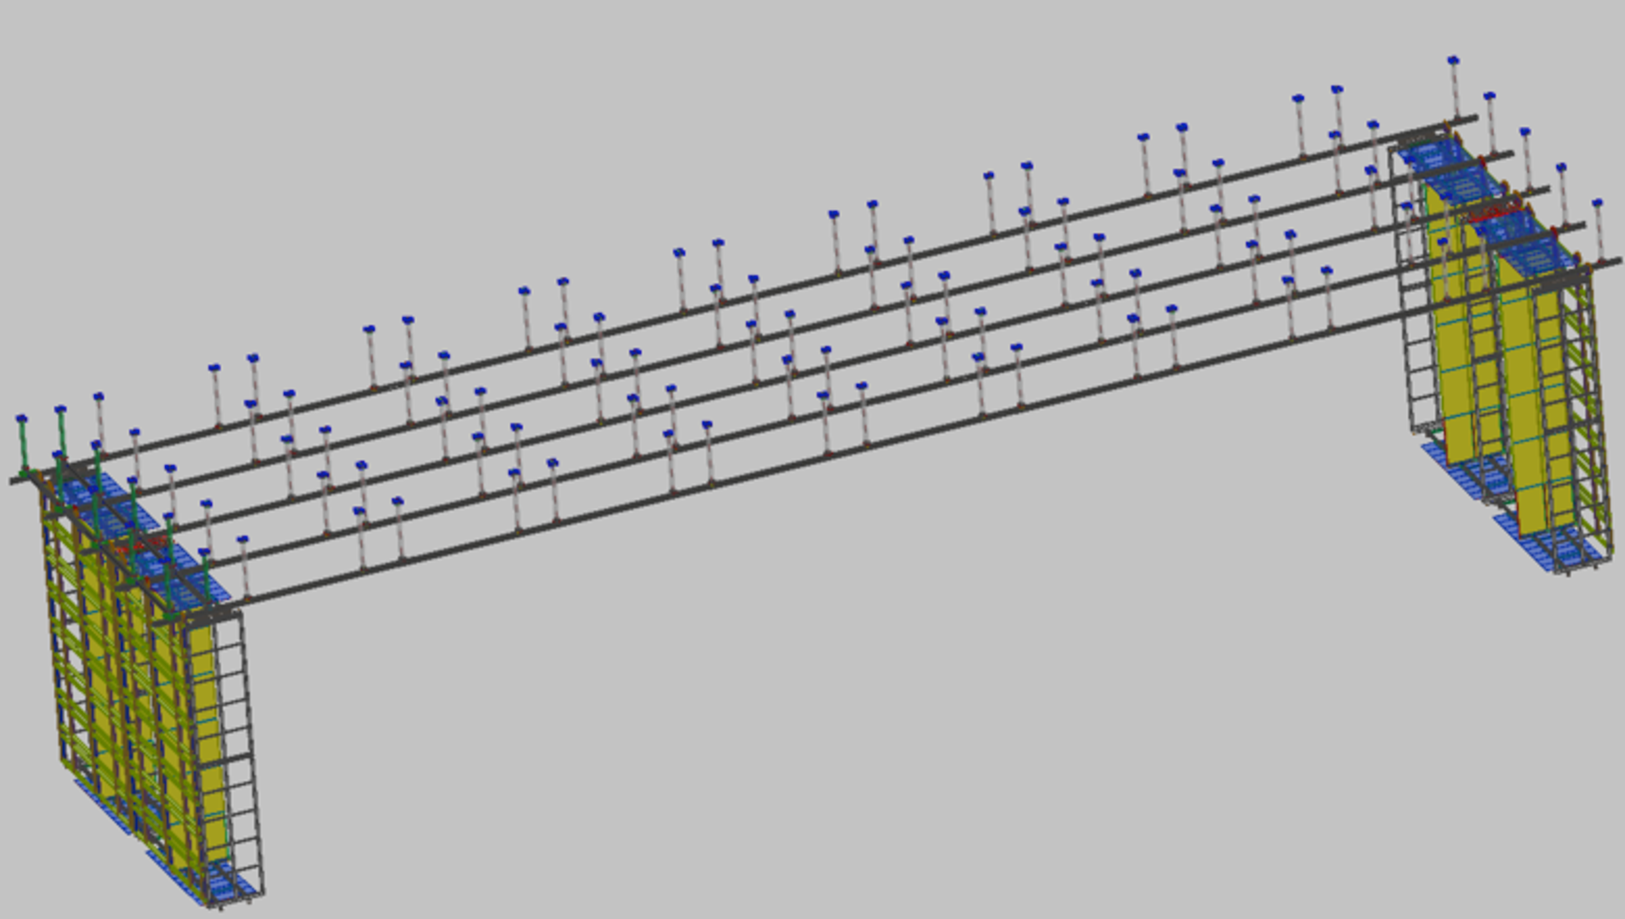
\includegraphics[width=\textwidth]{far-detector-single-phase/figures/DSS-1.pdf}
\end{minipage}
\begin{minipage}[c]{0.49\textwidth}
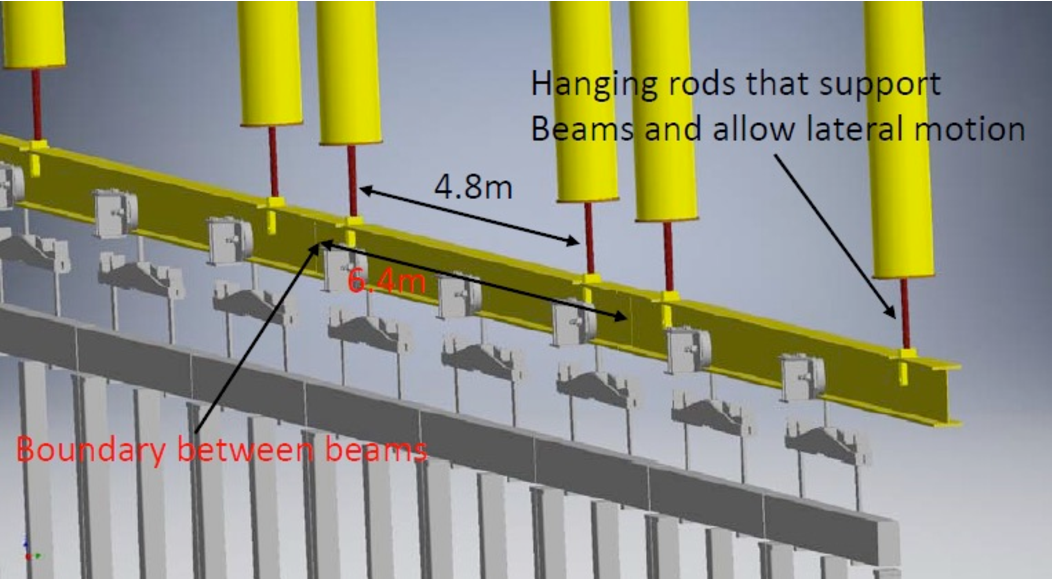
\includegraphics[width=\textwidth]{far-detector-single-phase/figures/DSS-2.pdf}
\end{minipage}
\caption{3-D model of the Detector Support System showing the entire structure on the left along with one row of \dword{apa} and \dword{cpa}/FC at each end. The right panel is a zoomed image showing the connections between the vertical supports and the horizontal I-beams.}
\label{DSS}
\end{center}
\end{figure}


Detector components will be installed using a shuttle beam system
illustrated in Fig.~\ref{shuttle}.  The last two columns of
feedthroughs (eastern most) will support temporary beams that run
north-south, perpendicular to the main DSS beams.  A shuttle beam
%shown in orange
will have trolleys mounted to it and will transverse
north-south until aligned with the required row of DSS beam.  The last
\dword{apa} or \dword{cpa} in a row is supported by the shuttle beam which is bolted
directly to the feedthroughs once it is in place.  As the last \dword{cpa} or
\dword{apa} in each row is installed the north-south beams are removed.

There will be a mechanical interlock system that prevents trolleys
from passing the end of the shuttle beam unless it is aligned with a
corresponding DSS beam.  The shuttle beam and each detector will be
moved using a motorized trolley.  A commercially available motorized
trolley will be modified as needed to meet the needs of the
installation.
\begin{figure}[htbp]
\begin{center}
\begin{minipage}[c]{0.49\textwidth}
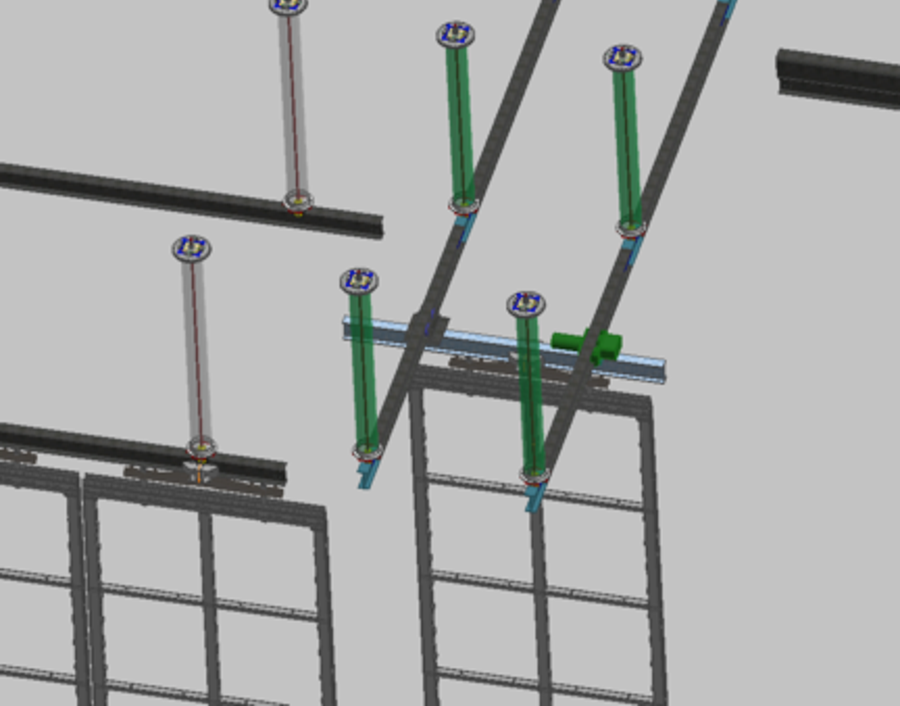
\includegraphics[width=\textwidth]{far-detector-single-phase/figures/Shuttle-1.pdf}
\end{minipage}
\begin{minipage}[c]{0.42\textwidth}
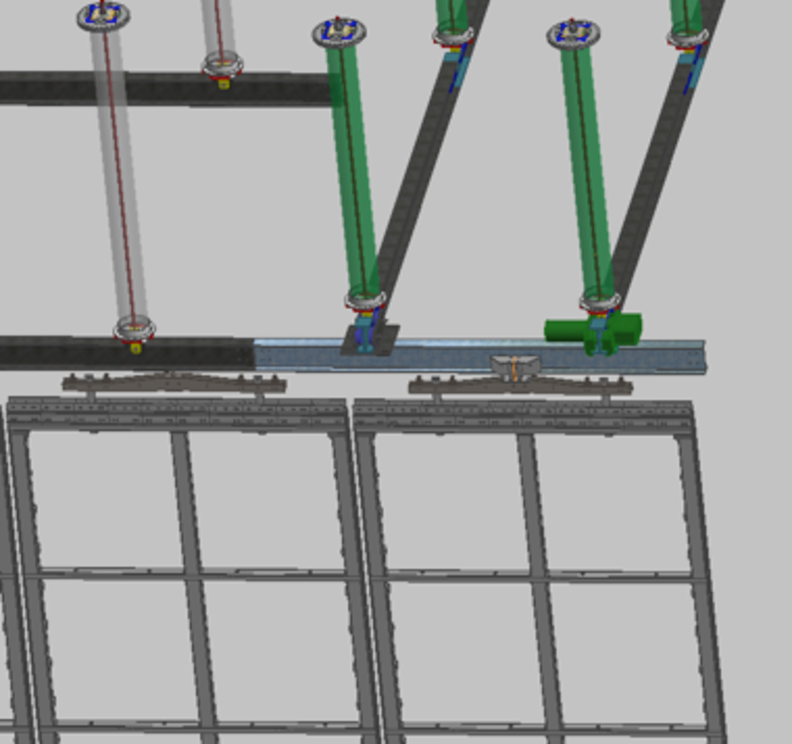
\includegraphics[width=\textwidth]{far-detector-single-phase/figures/shuttle-2.pdf}
\end{minipage}
\caption{3-D models of the shuttle beam end of the DSS. The figures show how an \dword{apa}
is translated into position using he North-South beams until it lines up with the correct
row of I-beams.}
\label{shuttle}
\end{center}
\end{figure}

The DSS installation begins with the placement and alignment of all
the feedthroughs onto the flanges that are mounted to the warm vessel.
There are \num{25} feedthroughs per row and five rows for a total of \num{125}
feedthroughs.  A fixture with a tooling ball will be attached to the
clevis of each feedthrough.  The $XY$ position in the horizontal plane
and the vertical $Z$ position of this tooling ball will be defined.  A
survey will be performed to determine the location of each tooling
ball center and $XY$ and $Z$ adjustments will be made to get the tooling
ball centers to within $\pm$\SI{3}{mm}.  The \SI{6.4}{m} long I-beams will then be
raised and pinned to the clevis.  Each beam weights roughly 350~lbs.
A lifting tripod will be placed over each of the feedthroughs
supporting a beam and a $1/4 ^{''}$ cable will be fed through the top
flange of the feedthrough down the \SI{14}{m} to the cryostat floor where it
will be attached to the I-beam.  The winches on each tripod will raise
the beam in unison in order to get it to the correct height to be
pinned to the feedthrough clevis.  Once the beams are mounted a final
survey of the beams will occur to ensure they are located and aligned
to each other properly.

A mock up of the shuttle system will be constructed to test the
mechanical interlock and drive systems for the shuttle beam
for each detector.  Tests will be conducted to evaluate the level of
misalignment between beams that can be tolerated and the amount of
positional control that can be achieved with the motorized trolley. It
is expected this will be finished prior to the TDR. At the time of the
TDR a larger prototype installation at Ash River will be under
construction. This prototype will use full scale elements and will be
used to develop the installation procedures and to also test the
detector installation process.


\subsection{Preparation for Operations}

After the \dwords{detmodule} are installed in the cryostats there remains a lot
of work before they can be operated. First the \dword{tco}
must be closed. This requires bringing back the cryostat manufacturer. 
First the missing panel with the steel beams
and steel panel are installed to complete the cryostat's outer
structural hull. Then the remaining foam blocks and membrane panels
are installed from the inside using the roof access holes 
to enter the cryostat. 

In parallel, the \lar pumps are installed at
the ends of the cryostat and final connections are made to the
recirculation plant. Once the pumps are installed, the cryostat is
closed, and everything is leak tested, the cryogenics plant can be
brought into operation. First the air inside the cryostat is purged by
injecting pure argon gas at the bottom %of the detector 
at a rate such
that the %detector 
cryostat volume is filled uniformly but faster than the diffusion
rate. This produces a column of argon gas that rises through the volume %detector
and sweeps out the air. This process is referred to as the \textit{piston
purge}. When the piston purge is complete the cool-down of the \dword{detmodule}
can begin. Misting nozzles inject a liquid-gas mix into the cryostat
that cools the detector components at a controlled rate. 

Once the detector is
cold the filling process can begin. Gaseous argon stored at the surface 
at \surf is brought down the shaft and is re-condensed underground. The \lar then flows through filters to remove any H$_2$O or O$_2$ and
flows into the cryostat. Given the very large volume of the cryostats
and the limited cooling power for re-condensing, it is  %the liquid is
expected to take \num{12} months to fill the first \dword{detmodule} and \num{14} months to
fill the second. During this time the detector readout electronics
will be on monitoring the status of the detector. % so the status of the detector can be monitored. 
Once the
\dword{detmodule} is full, the drift high voltage can be carefully ramped up and
data taking can begin.


